\documentclass[12pt,table,xcolor={dvipsnames}]{beamer}
\usetheme{Pittsburgh}
\usecolortheme{seagull}
%\usepackage[utf8]{inputenc}
\usepackage{fontspec}
\usepackage[brazilian]{babel}
\usepackage{amsmath}
\usepackage{listings}
\usepackage{tikz}
\usetikzlibrary{calc,shapes.multipart,chains,arrows, positioning, automata}
\usepackage{multirow}
\usepackage{amsfonts}
\usepackage{amssymb}
\usepackage{lstlinebgrd}
\usepackage{graphicx}
\author{Árvores AVL}
\title{Estruturas de Dados}
%\setbeamercovered{transparent}
\setbeamertemplate{navigation symbols}{}
%\logo{\includegraphics[scale=0.015]{Brasao_UFSC.png}
\includegraphics[scale=0.2]{brasao_PPGCC.jpg}}
\institute{Departamento de Informática e de Estatística \\ Prof. Jean Everson Martina \\ Prof. Aldo von Wangenheim}
\date{2016.2}
\subject{}
\usebackgroundtemplate{
\includegraphics[width=\paperwidth,
height=\paperheight]{../reusable_images/fundo_UFSC.png}}
\begin{document}

{
\usebackgroundtemplate{
\includegraphics[width=\paperwidth,
height=\paperheight]{../reusable_images/fundo_capa.png}}
\begin{frame}
\titlepage

\includegraphics[scale=0.3]{../reusable_images/brasao_INE.png}
\end{frame}
}

\begin{frame}[fragile]{Histórico}
\lstset{language=C++,
          keywordstyle=\color{blue}\ttfamily,
          stringstyle=\color{red}\ttfamily,
          commentstyle=\color{OliveGreen}\ttfamily,
          breaklines=true,
          basicstyle=\ttfamily\footnotesize
          }
\begin{columns}
\column{.5\textwidth}
\begin{block}{Árvore AVL}
Inventada em por Georgy Maximovich Adelson-Velskii e Yevgeniy Mikhailovich Landis ) e publicada em: "An algorithm for the organization of information. Trans. of Akademiya Nauk SSSR. Doklady, 1962, v. 146, no. 2, pp. 263-266 " 
\end{block}
\column{.5\textwidth}
\begin{center}
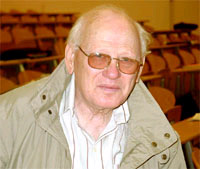
\includegraphics[scale=0.3]{av.png}\\ 
Georgy Maximovich Adelson-Velskii (Samara, Rússia, 1922)\\
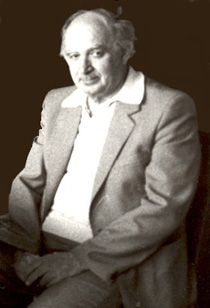
\includegraphics[scale=.2]{l.png}\\ 
Yevgeniy Mikhailovich Landis (Kharkov, Ucrânia, 1921)
\end{center}
\end{columns}          
\end{frame}

\begin{frame}[fragile]{Características}
\lstset{language=C++,
          keywordstyle=\color{blue}\ttfamily,
          stringstyle=\color{red}\ttfamily,
          commentstyle=\color{OliveGreen}\ttfamily,
          breaklines=true,
          basicstyle=\ttfamily\footnotesize
          }
\begin{itemize}
\item Manter uma árvore binária de busca balanceada sob a presença de constantes inserções e deleções é \textbf{ineficiente};
\item Para contornar esse problema foi criada a árvore \textbf{AVL (Adelson-Velskii e Landis)};
\item A árvore AVL é uma árvore binária com uma \textbf{condição de balanço}, porém não completamente balanceada;
\item Árvores AVL permitem inserção / deleção e \textbf{rebalanceamento} aceitavelmente rápidos.
\end{itemize}
\end{frame}

\begin{frame}[fragile]{Características}
\lstset{language=C++,
          keywordstyle=\color{blue}\ttfamily,
          stringstyle=\color{red}\ttfamily,
          commentstyle=\color{OliveGreen}\ttfamily,
          breaklines=true,
          basicstyle=\ttfamily\footnotesize
          }
\begin{itemize}
\item Critério de balanceamento:
\begin{itemize}
\item Dado um nodo qualquer, uma árvore está \textbf{AVL-balanceada} se as alturas das duas subárvores deste nodo diferem de, no máximo, 1;
\end{itemize}
\item Para rebalancear uma árvore após uma inserção, são utilizadas \textbf{rotações} de subárvores:
\begin{itemize}
\item Rotações simples em muitos casos;
\item Rotações duplas em alguns.
\end{itemize}
\end{itemize}
\end{frame}

\begin{frame}[fragile]{Características}
\lstset{language=C++,
          keywordstyle=\color{blue}\ttfamily,
          stringstyle=\color{red}\ttfamily,
          commentstyle=\color{OliveGreen}\ttfamily,
          breaklines=true,
          basicstyle=\ttfamily\footnotesize
          }
\begin{itemize}
\item Estrutura de um nodo na árvore AVL 
\begin{lstlisting}
Class nodoAVL {         
 info    :	tipo_info;
 esq     :	*nodoAVL;    
 dir     :	*nodoAVL;     
 alt     : 	inteiro; 
};
\end{lstlisting}
\item O campo \textbf{alt} deve ser atualizado recursivamente quando um nodo for inserido ou deletado.
\end{itemize}
\end{frame}

\begin{frame}[fragile]{Características}
\lstset{language=C++,
          keywordstyle=\color{blue}\ttfamily,
          stringstyle=\color{red}\ttfamily,
          commentstyle=\color{OliveGreen}\ttfamily,
          breaklines=true,
          basicstyle=\ttfamily\footnotesize
          }
\begin{itemize}
\item Para o retorno da altura de uma subárvore necessitamos de um método especial;
\item Um nodo pode não ter um ou ambos os filhos;
\item Lembre-se que a pesquisa para garantir a condição-AVL é realizada perguntando-se a altura das duas subárvores.
\begin{lstlisting}
inteiro altura( subárvore *nodoAVL) 
início                 
 se (subárvore for NULO)                         
  retorne -1; /* A altura de uma subárvore 
              inexistente é definida como -1 */
 senão                         
  retorne subárvore->alt;                 
 fim se         
fim
\end{lstlisting}
\end{itemize}
\end{frame}

\begin{frame}[fragile]{Inclusão com rotação}
\lstset{language=C++,
          keywordstyle=\color{blue}\ttfamily,
          stringstyle=\color{red}\ttfamily,
          commentstyle=\color{OliveGreen}\ttfamily,
          breaklines=true,
          basicstyle=\ttfamily\footnotesize
          }
          \tikzset{
  treenode/.style = {align=center, inner sep=0pt, text centered,
    font=\sffamily},
  node_b/.style = {treenode, circle, white, font=\sffamily\bfseries, draw=black,
    fill=black, text width=1.5em},
  node_r/.style = {treenode, circle, red, draw=red, 
    text width=1.5em, very thick},
  node_g/.style = {treenode, circle, green, draw=green, 
    text width=1.5em, very thick},
  node_s/.style = {treenode, circle, black, draw=black, 
    text width=1.5em, very thick},
  node_nil/.style = {treenode, rectangle, draw=black,
    minimum width=0.5em, minimum height=0.5em}
}
		  Exemplo de rebalanceamento:
          \begin{itemize}
          \item O nodo com chave 6.5 desequilibrou a árvore no nodo 8. Com a rotação da subárvore em torno do nodo 7, rebalanceamos.
          \end{itemize}
\begin{columns}
\column{.45\textwidth}
\begin{tikzpicture}[->,>=stealth',level/.style={sibling distance = 3cm/#1, level distance = 1.2cm}] 
\node [node_s] {6}
   child{ node [node_s] {2}
	   child{ node [node_s] {1}}
   	   child{ node [node_s] {4}
		 child{ node [node_s] {3}}  	   
		 child[missing]{ node [node_s] {}}
   	   }
   }
   child{ node [node_g] {8}
	   child{ node [node_s] {7} 
    	   child{ node [node_s] {6.5}} 
    	   child[missing]{ node [node_nil] {}}
	   } 
	   child[missing]{ node [node_nil] {}}  
   }
; 
\end{tikzpicture}
\column{.1\textwidth}
{\color{red} $\rightarrow$}
\column{.45\textwidth}
\begin{tikzpicture}[->,>=stealth',level/.style={sibling distance = 3cm/#1, level distance = 1.2cm}] 
\node [node_s] {6}
   child{ node [node_s] {2}
	   child{ node [node_s] {1}}
   	   child{ node [node_s] {4}
		 child{ node [node_s] {3}}  	   
		 child[missing]{ node [node_s] {}}
   	   }
   }
   child{ node [node_s] {7}
	   child{ node [node_s] {6.5} } 
	   child{ node [node_s] {8}}  
   }
; 
\end{tikzpicture}
\end{columns}         
\end{frame} 

\begin{frame}[fragile]{Inclusão com rotação}
\lstset{language=C++,
          keywordstyle=\color{blue}\ttfamily,
          stringstyle=\color{red}\ttfamily,
          commentstyle=\color{OliveGreen}\ttfamily,
          breaklines=true,
          basicstyle=\ttfamily\footnotesize
          }
          \tikzset{
  treenode/.style = {align=center, inner sep=0pt, text centered,
    font=\sffamily},
  node_b/.style = {treenode, circle, white, font=\sffamily\bfseries, draw=black,
    fill=black, text width=1.5em},
  node_r/.style = {treenode, circle, red, draw=red, 
    text width=1.5em, very thick},
  node_g/.style = {treenode, circle, green, draw=green, 
    text width=1.5em, very thick},
  node_s/.style = {treenode, circle, black, draw=black, 
    text width=1.5em, very thick},
  node_nil/.style = {treenode, rectangle, draw=black,
    minimum width=0.5em, minimum height=0.5em}
}
Algoritmo básico:
\begin{itemize}
\item Partimos do nodo inserido e subimos a árvore;
\item Atualizamos a informação do balanceamento em cada nodo (na árvore AVL, cada nodo conhece a sua altura);
\item Se chegamos à raiz sem encontrar nada errado, terminamos;
\item Saso encontremos um nodo desbalanceado  \textbf{(|altesq - altdir| < 2 ferida)}, realizamos a rotação no primeiro nodo desbalanceado encontrado;
\item No exemplo anterior, isto significa que, depois da inserção de 6.5, o nodo 8 ficou desbalanceado.
\end{itemize}      
\end{frame} 

\begin{frame}[fragile]{Exemplo: Adicionando de 1 a 7}
\lstset{language=C++,
          keywordstyle=\color{blue}\ttfamily,
          stringstyle=\color{red}\ttfamily,
          commentstyle=\color{OliveGreen}\ttfamily,
          breaklines=true,
          basicstyle=\ttfamily\footnotesize
          }
          \tikzset{
  treenode/.style = {align=center, inner sep=0pt, text centered,
    font=\sffamily},
  node_b/.style = {treenode, circle, white, font=\sffamily\bfseries, draw=black,
    fill=black, text width=1.5em},
  node_r/.style = {treenode, circle, red, draw=red, 
    text width=1.5em, very thick},
  node_g/.style = {treenode, circle, green, draw=green, 
    text width=1.5em, very thick},
  node_s/.style = {treenode, circle, black, draw=black, 
    text width=1.5em, very thick},
  node_nil/.style = {treenode, rectangle, draw=black,
    minimum width=0.5em, minimum height=0.5em}
}
          \begin{itemize}
          \item O primeiro problema ocorre quando inserimos o 3;
          \item A condição-AVL foi violada;
		  \item Executamos uma rotação simples entre a raiz (cuja condição-AVL está violada) e seu filho da direita.
          \end{itemize}
\begin{columns}
\column{.45\textwidth}
\begin{center}
\begin{tikzpicture}[->,>=stealth',level/.style={sibling distance = 1.5cm/#1, level distance = 1.2cm}] 
\node [node_s] {1}
   child[missing]{ node [node_s] {}}
   child{ node [node_s] {2}
    child[missing]{ node [node_s] {}}
    child{ node [node_g] {3}}
   }
; 
\end{tikzpicture}
\end{center}
\column{.1\textwidth}
{\color{red} $\rightarrow$}
\column{.45\textwidth}
\begin{center}
\begin{tikzpicture}[->,>=stealth',level/.style={sibling distance = 1.5cm/#1, level distance = 1.2cm}] 
\node [node_s] {2}
   child {node [node_s] {1}}
   child {node [node_s] {3}}

; 
\end{tikzpicture}
\end{center}
\end{columns}         
\end{frame} 

\begin{frame}[fragile]{Exemplo: Adicionando de 1 a 7}
\lstset{language=C++,
          keywordstyle=\color{blue}\ttfamily,
          stringstyle=\color{red}\ttfamily,
          commentstyle=\color{OliveGreen}\ttfamily,
          breaklines=true,
          basicstyle=\ttfamily\footnotesize
          }
          \tikzset{
  treenode/.style = {align=center, inner sep=0pt, text centered,
    font=\sffamily},
  node_b/.style = {treenode, circle, white, font=\sffamily\bfseries, draw=black,
    fill=black, text width=1.5em},
  node_r/.style = {treenode, circle, red, draw=red, 
    text width=1.5em, very thick},
  node_g/.style = {treenode, circle, green, draw=green, 
    text width=1.5em, very thick},
  node_s/.style = {treenode, circle, black, draw=black, 
    text width=1.5em, very thick},
  node_nil/.style = {treenode, rectangle, draw=black,
    minimum width=0.5em, minimum height=0.5em}
}
          \begin{itemize}
          \item Inserimos o elemento 4 sem problemas;
		  \item Inserimos o elemento 5: violação em 3;
		  \item Mesmo processo da rotação anterior será seguido;
		  \item Importantíssimo: observe-se que 2 precisa ser notificado que seu filho agora é o nodo com chave 4.
          \end{itemize}
\begin{columns}
\column{.45\textwidth}
\begin{center}
\begin{tikzpicture}[->,>=stealth',level/.style={sibling distance = 1.5cm/#1, level distance = 1.2cm}] 
\node [node_s] {2}
   child {node [node_s] {1}}
   child {node [node_g] {3}
    child [missing]{node [node_s] {}}
    child {node [node_s] {4}
     child [missing]{node [node_s] {}}
     child {node [node_s] {5}}
    }
   }

; 
\end{tikzpicture}
\end{center}
\column{.1\textwidth}
{\color{red} $\rightarrow$}
\column{.45\textwidth}
\begin{center}
\begin{tikzpicture}[->,>=stealth',level/.style={sibling distance = 2cm/#1, level distance = 1.2cm}] 
\node [node_s] {2}
   child {node [node_s] {1}}
   child {node [node_s] {4}
    child {node [node_s] {3}}
    child {node [node_s] {5}}
   }

; 
\end{tikzpicture}
\end{center}
\end{columns}         
\end{frame} 

\begin{frame}[fragile]{Exemplo: Adicionando de 1 a 7}
\lstset{language=C++,
          keywordstyle=\color{blue}\ttfamily,
          stringstyle=\color{red}\ttfamily,
          commentstyle=\color{OliveGreen}\ttfamily,
          breaklines=true,
          basicstyle=\ttfamily\footnotesize
          }
          \tikzset{
  treenode/.style = {align=center, inner sep=0pt, text centered,
    font=\sffamily},
  node_b/.style = {treenode, circle, white, font=\sffamily\bfseries, draw=black,
    fill=black, text width=1.5em},
  node_r/.style = {treenode, circle, red, draw=red, 
    text width=1.5em, very thick},
  node_g/.style = {treenode, circle, green, draw=green, 
    text width=1.5em, very thick},
  node_s/.style = {treenode, circle, black, draw=black, 
    text width=1.5em, very thick},
  node_nil/.style = {treenode, rectangle, draw=black,
    minimum width=0.5em, minimum height=0.5em}
}
          \begin{itemize}
          \item A inclusão do elemento 6 desequilibra a raiz:
          \begin{itemize}
          \item subárvore direita tem altura 0;
		  \item subárvore esquerda tem altura 2;
          \end{itemize}
		  \item Rotacionamos na raiz entre 2 e 4.
          \end{itemize}
\begin{columns}
\column{.45\textwidth}
\begin{center}
\begin{tikzpicture}[->,>=stealth',level/.style={sibling distance = 2cm/#1, level distance = 1.2cm}] 
\node [node_g] {2}
   child {node [node_s] {1}}
   child {node [node_s] {4}
    child {node [node_s] {3}}
    child {node [node_s] {5}
     child [missing] {node [node_s] {}}
     child {node [node_s] {6}}    
    }
   }

; 
\end{tikzpicture}
\end{center}
\column{.1\textwidth}
{\color{red} $\rightarrow$}
\column{.45\textwidth}
\begin{center}
\begin{tikzpicture}[->,>=stealth',level/.style={sibling distance = 2cm/#1, level distance = 1.2cm}] 
\node [node_s] {4}
   child {node [node_s] {2}
    child {node [node_s] {1}}
    child {node [node_s] {3}}   
   }
   child {node [node_s] {5}
    child [missing] {node [node_s] {}}
    child {node [node_s] {6}}
   }

; 
\end{tikzpicture}
\end{center}
\end{columns}         
\end{frame} 

\begin{frame}[fragile]{Exemplo: Adicionando de 1 a 7}
\lstset{language=C++,
          keywordstyle=\color{blue}\ttfamily,
          stringstyle=\color{red}\ttfamily,
          commentstyle=\color{OliveGreen}\ttfamily,
          breaklines=true,
          basicstyle=\ttfamily\footnotesize
          }
          \tikzset{
  treenode/.style = {align=center, inner sep=0pt, text centered,
    font=\sffamily},
  node_b/.style = {treenode, circle, white, font=\sffamily\bfseries, draw=black,
    fill=black, text width=1.5em},
  node_r/.style = {treenode, circle, red, draw=red, 
    text width=1.5em, very thick},
  node_g/.style = {treenode, circle, green, draw=green, 
    text width=1.5em, very thick},
  node_s/.style = {treenode, circle, black, draw=black, 
    text width=1.5em, very thick},
  node_nil/.style = {treenode, rectangle, draw=black,
    minimum width=0.5em, minimum height=0.5em}
}
          \begin{itemize}
          \item A inclusão de um nodo com chave 7 causa uma rotação como já havíamos visto antes:
          \begin{itemize}
          \item O 5 fica desequilibrado;
          \item Rotacionamos em 6.
          \end{itemize}
          \end{itemize}
\begin{columns}
\column{.45\textwidth}
\begin{center}
\begin{tikzpicture}[->,>=stealth',level/.style={sibling distance = 2cm/#1, level distance = 1.2cm}] 
\node [node_s] {4}
   child {node [node_s] {2}
    child {node [node_s] {1}}
    child {node [node_s] {3}}   
   }
   child {node [node_g] {5}
    child [missing] {node [node_s] {}}
    child {node [node_s] {6}
     child [missing] {node [node_s] {}}
     child {node [node_s] {7}}    
    }
   }

; 
\end{tikzpicture}
\end{center}
\column{.1\textwidth}
{\color{red} $\rightarrow$}
\column{.45\textwidth}
\begin{center}
\begin{tikzpicture}[->,>=stealth',level/.style={sibling distance = 2cm/#1, level distance = 1.2cm}] 
\node [node_s] {4}
   child {node [node_s] {2}
    child {node [node_s] {1}}
    child {node [node_s] {3}}   
   }
   child {node [node_s] {6}
    child {node [node_s] {5}}
    child {node [node_s] {7}}
   }

; 
\end{tikzpicture}
\end{center}
\end{columns}         
\end{frame} 

\begin{frame}[fragile]{Inclusão com rotação simples à esquerda}
\lstset{language=C++,
          keywordstyle=\color{blue}\ttfamily,
          stringstyle=\color{red}\ttfamily,
          commentstyle=\color{OliveGreen}\ttfamily,
          breaklines=true,
          basicstyle=\ttfamily\footnotesize
          }
\begin{lstlisting}
nodoAVL *simp_roda_esq(k2 *nodoAVL)
variáveis locais
 k1 : *nodoAVL;
início
 k1 <- k2->esq;
 k2->esq <- k1->dir;
 k1->dir <- k2;
  /* atualize alturas */
 k2->alt <-max(altura(k2->esq),altura(k2->dir))+ 1;
 k1->alt <-max(altura(k1->esq),k2->alt) + 1;     
 retorne k1; /* nova raiz da subárvore */
fim
\end{lstlisting}
\end{frame}

\begin{frame}[fragile]{Inclusão com rotação simples à direita}
\lstset{language=C++,
          keywordstyle=\color{blue}\ttfamily,
          stringstyle=\color{red}\ttfamily,
          commentstyle=\color{OliveGreen}\ttfamily,
          breaklines=true,
          basicstyle=\ttfamily\footnotesize
          }
\begin{lstlisting}
nodoAVL *simp_roda_dir(k2 *nodoAVL)
variáveis locais
 k1 : *nodoAVL;
início
 k1 <- k2->dir;
 k2->dir <- k1->esq;
 k1->esq <- k2;
  /* atualize alturas */
 k2->alt <-max(altura(k2->dir),altura(k2->esq))+ 1;
 k1->alt <-max(altura(k1->dir),k2->alt) + 1;     
 retorne k1; /* nova raiz da subárvore */
fim
\end{lstlisting}
\end{frame}

\begin{frame}[fragile]{Inclusão com rotação dupla}
\lstset{language=C++,
          keywordstyle=\color{blue}\ttfamily,
          stringstyle=\color{red}\ttfamily,
          commentstyle=\color{OliveGreen}\ttfamily,
          breaklines=true,
          basicstyle=\ttfamily\footnotesize
          }
\begin{itemize}
\item O algoritmo descrito até agora tem um problema:
\begin{itemize}
\item Existem casos onde ele não basta para consertar a árvore após uma inclusão ou exclusão;
\end{itemize}
\item Exemplo: inserimos as chaves 8 a 15, em ordem inversa, na árvore anterior:
\begin{itemize}
\item A inserção de 15 não provoca problemas, nem desbalanceia a árvore;
\item A inserção de 14, por sua vez, faz o rebalanceamento falhar.
\end{itemize}
\end{itemize}
\end{frame}

\begin{frame}[fragile]{Rotação Simples Não é Suficiente}
\lstset{language=C++,
          keywordstyle=\color{blue}\ttfamily,
          stringstyle=\color{red}\ttfamily,
          commentstyle=\color{OliveGreen}\ttfamily,
          breaklines=true,
          basicstyle=\ttfamily\footnotesize
          }
          \tikzset{
  treenode/.style = {align=center, inner sep=0pt, text centered,
    font=\sffamily},
  node_b/.style = {treenode, circle, white, font=\sffamily\bfseries, draw=black,
    fill=black, text width=1.5em},
  node_r/.style = {treenode, circle, red, draw=red, 
    text width=1.5em, very thick},
  node_g/.style = {treenode, circle, green, draw=green, 
    text width=1.5em, very thick},
  node_s/.style = {treenode, circle, black, draw=black, 
    text width=1.5em, very thick},
  node_nil/.style = {treenode, rectangle, draw=black,
    minimum width=0.5em, minimum height=0.5em}
}
          \begin{itemize}
          \item O problema que surge aqui é que tanto 7 como 14 são candidatos à subárvore esquerda de 15.
		  \item Neste caso, necessitamos de uma dupla rotação.
          \end{itemize}
\begin{columns}
\column{.45\textwidth}
\begin{center}
\begin{tikzpicture}[->,>=stealth',level/.style={sibling distance = 2cm/#1, level distance = 1.2cm}] 
\node [node_s] {4}
   child {node [node_s] {2}
    child {node [node_s] {1}}
    child {node [node_s] {3}}   
   }
   child {node [node_s] {6}
    child {node [node_s] {5}}
    child {node [node_g] {7}
     child [missing] {node [node_s] {}}
     child {node [node_s] {15}
      child {node [node_s] {14}}
      child [missing] {node [node_s] {}}
     }
    }
   }
; 
\end{tikzpicture}
\end{center}
\column{.1\textwidth}
{\color{red} $\rightarrow$}
\column{.45\textwidth}
\begin{center}
\begin{tikzpicture}[->,>=stealth',level/.style={sibling distance = 2cm/#1, level distance = 1.2cm}] 
\node [node_s] {4}
   child {node [node_s] {2}
    child {node [node_s] {1}}
    child {node [node_s] {3}}   
   }
   child {node [node_s] {6}
    child {node [node_s] {5}}
    child {node [node_g] {15}
     child {node [node_s] {7}
      child [missing] {node [node_s] {}}     
      child {node [node_s] {14}}      
     }    
     child [missing] {node [node_s] {}}     
    }
   }
; 
\end{tikzpicture}
\end{center}
\end{columns}         
\end{frame} 

\begin{frame}[fragile]{Inclusão com Rotação Dupla}
\lstset{language=C++,
          keywordstyle=\color{blue}\ttfamily,
          stringstyle=\color{red}\ttfamily,
          commentstyle=\color{OliveGreen}\ttfamily,
          breaklines=true,
          basicstyle=\ttfamily\footnotesize
          }
          \tikzset{
  treenode/.style = {align=center, inner sep=0pt, text centered,
    font=\sffamily},
  node_b/.style = {treenode, circle, white, font=\sffamily\bfseries, draw=black,
    fill=black, text width=1.5em},
  node_r/.style = {treenode, circle, red, draw=red, 
    text width=1.5em, very thick},
  node_g/.style = {treenode, circle, green, draw=green, 
    text width=1.5em, very thick},
  node_s/.style = {treenode, circle, black, draw=black, 
    text width=1.5em, very thick},
  node_nil/.style = {treenode, rectangle, draw=black,
    minimum width=0.5em, minimum height=0.5em}
}
          \begin{itemize}
          \item No exemplo, a rotação direita-esquerda envolve o 7, o 15 e o 14;
		  \item Primeiro rotacionamos 14-15 à direita, depois 7-14 à esquerda.
          \end{itemize}
\begin{columns}
\column{.45\textwidth}
\begin{center}
\begin{tikzpicture}[->,>=stealth',level/.style={sibling distance = 2cm/#1, level distance = 1.2cm}] 
\node [node_s] {4}
   child {node [node_s] {2}
    child {node [node_s] {1}}
    child {node [node_s] {3}}   
   }
   child {node [node_s] {6}
    child {node [node_s] {5}}
    child {node [node_g] {7}
     child [missing] {node [node_s] {}}
     child {node [node_s] {15}
      child {node [node_s] {14}}
      child [missing] {node [node_s] {}}
     }
    }
   }
; 
\end{tikzpicture}
\end{center}
\column{.1\textwidth}
{\color{red} $\rightarrow$}
\column{.45\textwidth}
\begin{center}
\begin{tikzpicture}[->,>=stealth',level/.style={sibling distance = 2cm/#1, level distance = 1.2cm}] 
\node [node_s] {4}
   child {node [node_s] {2}
    child {node [node_s] {1}}
    child {node [node_s] {3}}   
   }
   child {node [node_s] {6}
    child {node [node_s] {5}}
    child {node [node_g] {7}
     child [missing] {node [node_s] {}}
     child {node [node_s] {14}
      child [missing] {node [node_s] {}}
      child {node [node_s] {15}}
     }
    }
   }
; 
\end{tikzpicture}
\end{center}
\end{columns}         
\end{frame} 

\begin{frame}[fragile]{Inclusão com Rotação Dupla}
\lstset{language=C++,
          keywordstyle=\color{blue}\ttfamily,
          stringstyle=\color{red}\ttfamily,
          commentstyle=\color{OliveGreen}\ttfamily,
          breaklines=true,
          basicstyle=\ttfamily\footnotesize
          }
          \tikzset{
  treenode/.style = {align=center, inner sep=0pt, text centered,
    font=\sffamily},
  node_b/.style = {treenode, circle, white, font=\sffamily\bfseries, draw=black,
    fill=black, text width=1.5em},
  node_r/.style = {treenode, circle, red, draw=red, 
    text width=1.5em, very thick},
  node_g/.style = {treenode, circle, green, draw=green, 
    text width=1.5em, very thick},
  node_s/.style = {treenode, circle, black, draw=black, 
    text width=1.5em, very thick},
  node_nil/.style = {treenode, rectangle, draw=black,
    minimum width=0.5em, minimum height=0.5em}
}
          \begin{itemize}
          \item No exemplo, a rotação direita-esquerda envolve o 7, o 15 e o 14;
		  \item Primeiro rotacionamos 14-15 à direita, depois 7-14 à esquerda.
          \end{itemize}
\begin{columns}
\column{.45\textwidth}
\begin{center}
\begin{tikzpicture}[->,>=stealth',level/.style={sibling distance = 2cm/#1, level distance = 1.2cm}] 
\node [node_s] {4}
   child {node [node_s] {2}
    child {node [node_s] {1}}
    child {node [node_s] {3}}   
   }
   child {node [node_s] {6}
    child {node [node_s] {5}}
    child {node [node_g] {7}
     child [missing] {node [node_s] {}}
     child {node [node_s] {14}
      child [missing] {node [node_s] {}}
      child {node [node_s] {15}}
     }
    }
   }
; 
\end{tikzpicture}
\end{center}
\column{.1\textwidth}
{\color{red} $\rightarrow$}
\column{.45\textwidth}
\begin{center}
\begin{tikzpicture}[->,>=stealth',level/.style={sibling distance = 2cm/#1, level distance = 1.2cm}] 
\node [node_s] {4}
   child {node [node_s] {2}
    child {node [node_s] {1}}
    child {node [node_s] {3}}   
   }
   child {node [node_s] {6}
    child {node [node_s] {5}}
    child {node [node_s] {14}
     child {node [node_s] {7}}
     child {node [node_s] {15}}
    }
   }
; 
\end{tikzpicture}
\end{center}
\end{columns}         
\end{frame} 

\begin{frame}[fragile]{Inclusão do Elemento 13}
\lstset{language=C++,
          keywordstyle=\color{blue}\ttfamily,
          stringstyle=\color{red}\ttfamily,
          commentstyle=\color{OliveGreen}\ttfamily,
          breaklines=true,
          basicstyle=\ttfamily\footnotesize
          }
          \tikzset{
  treenode/.style = {align=center, inner sep=0pt, text centered,
    font=\sffamily},
  node_b/.style = {treenode, circle, white, font=\sffamily\bfseries, draw=black,
    fill=black, text width=1.5em},
  node_r/.style = {treenode, circle, red, draw=red, 
    text width=1.5em, very thick},
  node_g/.style = {treenode, circle, green, draw=green, 
    text width=1.5em, very thick},
  node_s/.style = {treenode, circle, black, draw=black, 
    text width=1.5em, very thick},
  node_nil/.style = {treenode, rectangle, draw=black,
    minimum width=0.5em, minimum height=0.5em}
}
          \begin{itemize}
          \item Novamente uma dupla rotação direita-esquerda.
          \end{itemize}
\begin{columns}
\column{.45\textwidth}
\begin{center}
\begin{tikzpicture}[->,>=stealth',level/.style={sibling distance = 2cm/#1, level distance = 1.2cm}] 
\node [node_s] {4}
   child {node [node_s] {2}
    child {node [node_s] {1}}
    child {node [node_s] {3}}   
   }
   child {node [node_g] {6}
    child {node [node_s] {5}}
    child {node [node_s] {14}
     child {node [node_s] {7}}
     child {node [node_s] {15}
      child [missing] {node [node_s] {}}
      child {node [node_s] {13}}
     }
    }
   }
; 
\end{tikzpicture}
\end{center}
\column{.1\textwidth}
{\color{red} $\rightarrow$}
\column{.45\textwidth}
\begin{center}
\begin{tikzpicture}[->,>=stealth',level/.style={sibling distance = 2cm/#1, level distance = 1.2cm}] 
\node [node_s] {4}
   child {node [node_s] {2}
    child {node [node_s] {1}}
    child {node [node_s] {3}}   
   }
   child {node [node_s] {7}
    child {node [node_s] {6}
     child {node [node_s] {5}}
     child [missing] {node [node_s] {}}    
    }
    child {node [node_s] {14}
     child {node [node_s] {13}}
     child {node [node_s] {15}}
    }
   }
; 
\end{tikzpicture}
\end{center}
\end{columns}         
\end{frame}

\begin{frame}[fragile]{Inclusão do Elemento 12}
\lstset{language=C++,
          keywordstyle=\color{blue}\ttfamily,
          stringstyle=\color{red}\ttfamily,
          commentstyle=\color{OliveGreen}\ttfamily,
          breaklines=true,
          basicstyle=\ttfamily\footnotesize
          }
          \tikzset{
  treenode/.style = {align=center, inner sep=0pt, text centered,
    font=\sffamily},
  node_b/.style = {treenode, circle, white, font=\sffamily\bfseries, draw=black,
    fill=black, text width=1.5em},
  node_r/.style = {treenode, circle, red, draw=red, 
    text width=1.5em, very thick},
  node_g/.style = {treenode, circle, green, draw=green, 
    text width=1.5em, very thick},
  node_s/.style = {treenode, circle, black, draw=black, 
    text width=1.5em, very thick},
  node_nil/.style = {treenode, rectangle, draw=black,
    minimum width=0.5em, minimum height=0.5em}
}
          \begin{itemize}
          \item A inclusão do elemento 12 provoca um desequilíbrio na raiz;
          \item Mas agora é simples.
          \end{itemize}
\begin{columns}
\column{.45\textwidth}
\begin{center}
\begin{tikzpicture}[->,>=stealth',level/.style={sibling distance = 2cm/#1, level distance = 1.2cm}] 
\node [node_g] {4}
   child {node [node_s] {2}
    child {node [node_s] {1}}
    child {node [node_s] {3}}   
   }
   child {node [node_s] {7}
    child {node [node_s] {6}
     child {node [node_s] {5}}
     child [missing] {node [node_s] {}}    
    }
    child {node [node_s] {14}
     child {node [node_s] {13}
      child {node [node_s] {12}}
      child [missing] {node [node_s] {}}    
     }
     child {node [node_s] {15}}
    }
   }
; 
\end{tikzpicture}
\end{center}
\column{.1\textwidth}
{\color{red} $\rightarrow$}
\column{.6\textwidth}
\begin{center}
\begin{tikzpicture}[->,>=stealth',level/.style={sibling distance = 3.5cm/#1, level distance = 1cm}] 
\node [node_s] {7}
   child {node [node_s] {4}
    child {node [node_s] {2}
     child {node [node_s] {1}}
     child {node [node_s] {3}}      
    }
    child {node [node_s] {6}
     child {node [node_s] {5}}
     child [missing] {node [node_s] {}}      
    }   
   }
   child {node [node_s] {14}
    child {node [node_s] {13}
     child {node [node_s] {12}}
     child [missing] {node [node_s] {}}      
    }
    child {node [node_s] {15}}
   }
; 
\end{tikzpicture}
\end{center}
\end{columns}         
\end{frame}

\begin{frame}[fragile]{Rotação Dupla à Esquerda}
\lstset{language=C++,
          keywordstyle=\color{blue}\ttfamily,
          stringstyle=\color{red}\ttfamily,
          commentstyle=\color{OliveGreen}\ttfamily,
          breaklines=true,
          basicstyle=\ttfamily\footnotesize
          }
\begin{itemize}
\item Função chamada somente se k3 possuir um filho à esquerda e se o filho à esquerda de k3 possuir um filho à direita. Ela realiza a rotação e atualiza as alturas das subárvores rotacionadas.
\begin{lstlisting}
nodoAVL *dup_roda_esq(k3 : *nodoAVL) 
início                 
 /* Rotacione entre k1 e k2 */                 
 k3->esq <- simp_roda_dir( k3-> esq );
 /* Rotacione entre k3 e k2 */                 
 retorne ( simp_roda_esq( k3 );         
fim 
\end{lstlisting}
\item Da mesma forma que com a rotação simples, a rotação dupla à direita é a operação simétrica da rotação à esquerda e é facilmente implementada. 
\end{itemize}
\end{frame}

\begin{frame}[fragile]{Inserção em Árvore AVL}
\lstset{language=C++,
          keywordstyle=\color{blue}\ttfamily,
          stringstyle=\color{red}\ttfamily,
          commentstyle=\color{OliveGreen}\ttfamily,
          breaklines=true,
          escapeinside={(*@}{@*)},
          basicstyle=\ttfamily\scriptsize
          }
\begin{lstlisting}
nodoAVL *inserçãoAVL(T* info, *nodoAVL arv, *nodoAVL pai)
variáveis
 arv_rodada : *nodoAVL;
início
 se (arv é NULO) então /* Folha: aloca novo nodo */
  arv <- aloca novo nodo;
  se (arv é NULO) então retorne ERRO;
  arv->info <- info;	arv->alt <- 0;
  arv->esq <- NULO;	arv->dir <- NULO;
 senão
  se (info < arv->info) então
   arv->esq <- inserçãoAVL(info, arv->esq, arv);
   se ((altura(arv->esq) - altura(arv->dir) > 1)
    se (info < arv->esq->info) então 
     arv_rodada<-simp_roda_esq(arv);
    senão arv_rodada <- dup_roda_esq(arv);
    fim se
    se (pai->esq = arv) então pai->esq <- arv_rodada;
    senão pai->dir <- arv_rodada;
    fim se
   senão
    arv->alt <- max( altura(arv->esq), altura(arv->dir)) + 1;
   fim se
  senão // (continua)
  (*@  \textcolor{red}{}  @*)
\end{lstlisting}
\end{frame}

\begin{frame}[fragile]{Inserção em Árvore AVL}
\lstset{language=C++,
          keywordstyle=\color{blue}\ttfamily,
          stringstyle=\color{red}\ttfamily,
          commentstyle=\color{OliveGreen}\ttfamily,
          breaklines=true,
          escapeinside={(*@}{@*)},
          basicstyle=\ttfamily\scriptsize
          }
\begin{lstlisting}
nodoAVL *inserçãoAVL(T* info, *nodoAVL arv, *nodoAVL pai)
variáveis
 arv_rodada : *nodoAVL;
início
 se (arv é NULO) então /* Folha: aloca novo nodo */
  arv <- aloca novo nodo;
  se (arv é NULO) então retorne ERRO;
  arv->info <- info;	arv->alt <- 0;
  arv->esq <- NULO;	arv->dir <- NULO;
 senão
  se (info < arv->info) então
   arv->esq <- inserçãoAVL(info, arv->esq, arv);
   (*@  \textcolor{red}{se ((altura(arv->esq) - altura(arv->dir) > 1)}  @*)
    (*@  \textcolor{red}{se (info < arv->esq->info) então }  @*)
     (*@  \textcolor{red}{arv\_rodada<-simp\_roda\_esq(arv);}  @*)
    (*@  \textcolor{red}{senão arv\_rodada <- dup\_roda\_esq(arv);}  @*)
    (*@  \textcolor{red}{fim se}  @*)
    (*@  \textcolor{red}{se (pai->esq = arv) então pai->esq <- arv\_rodada;}  @*)
    (*@  \textcolor{red}{senão pai->dir <- arv\_rodada;}  @*)
    (*@  \textcolor{red}{fim se}  @*)
   (*@  \textcolor{red}{senão}  @*)
    (*@  \textcolor{red}{arv->alt <- max( altura(arv->esq), altura(arv->dir)) + 1;}  @*)
   (*@  \textcolor{red}{fim se}  @*)
  senão // (continua)
  (*@  \textcolor{red}{}  @*)
\end{lstlisting}
\end{frame}

\begin{frame}[fragile]{Inserção em Árvore AVL}
\lstset{language=C++,
          keywordstyle=\color{blue}\ttfamily,
          stringstyle=\color{red}\ttfamily,
          commentstyle=\color{OliveGreen}\ttfamily,
          breaklines=true,
          escapeinside={(*@}{@*)},
          basicstyle=\ttfamily\scriptsize
          }
\begin{lstlisting}
nodoAVL *inserçãoAVL(T* info, *nodoAVL arv, *nodoAVL pai)
variáveis
 arv_rodada : *nodoAVL;
início
 se (arv é NULO) então /* Folha: aloca novo nodo */
  arv <- aloca novo nodo;
  se (arv é NULO) então retorne ERRO;
  arv->info <- info;	arv->alt <- 0;
  arv->esq <- NULO;	arv->dir <- NULO;
 senão
  se (info < arv->info) então
   arv->esq <- inserçãoAVL(info, arv->esq, arv);
   (*@  \textcolor{red}{se ((altura(arv->esq) - altura(arv->dir) > 1)}  @*)//Rotaciona?
    se (info < arv->esq->info) então 
     arv_rodada<-simp_roda_esq(arv);
    senão arv_rodada <- dup_roda_esq(arv);
    fim se
    se (pai->esq = arv) então pai->esq <- arv_rodada;
    senão pai->dir <- arv_rodada;
    fim se
   senão
    arv->alt <- max( altura(arv->esq), altura(arv->dir)) + 1;
   fim se
  senão // (continua)
  (*@  \textcolor{red}{}  @*)
\end{lstlisting}
\end{frame}

\begin{frame}[fragile]{Inserção em Árvore AVL}
\lstset{language=C++,
          keywordstyle=\color{blue}\ttfamily,
          stringstyle=\color{red}\ttfamily,
          commentstyle=\color{OliveGreen}\ttfamily,
          breaklines=true,
          escapeinside={(*@}{@*)},
          basicstyle=\ttfamily\scriptsize
          }
\begin{lstlisting}
nodoAVL *inserçãoAVL(T* info, *nodoAVL arv, *nodoAVL pai)
variáveis
 arv_rodada : *nodoAVL;
início
 se (arv é NULO) então /* Folha: aloca novo nodo */
  arv <- aloca novo nodo;
  se (arv é NULO) então retorne ERRO;
  arv->info <- info;	arv->alt <- 0;
  arv->esq <- NULO;	arv->dir <- NULO;
 senão
  se (info < arv->info) então
   arv->esq <- inserçãoAVL(info, arv->esq, arv);
   se ((altura(arv->esq) - altura(arv->dir) > 1)
    (*@  \textcolor{red}{se (info < arv->esq->info) então }  @*)//Qual Rotacão?
     (*@  \textcolor{red}{arv\_rodada<-simp\_roda\_esq(arv);}  @*)
    (*@  \textcolor{red}{senão arv\_rodada <- dup\_roda\_esq(arv);}  @*)
    (*@  \textcolor{red}{fim se}  @*)
    se (pai->esq = arv) então pai->esq <- arv_rodada;
    senão pai->dir <- arv_rodada;
    fim se
   senão
    arv->alt <- max( altura(arv->esq), altura(arv->dir)) + 1;
   fim se
  senão // (continua)
  (*@  \textcolor{red}{}  @*)
\end{lstlisting}
\end{frame}

\begin{frame}[fragile]{Inserção em Árvore AVL}
\lstset{language=C++,
          keywordstyle=\color{blue}\ttfamily,
          stringstyle=\color{red}\ttfamily,
          commentstyle=\color{OliveGreen}\ttfamily,
          breaklines=true,
          escapeinside={(*@}{@*)},
          basicstyle=\ttfamily\scriptsize
          }
\begin{lstlisting}
nodoAVL *inserçãoAVL(T* info, *nodoAVL arv, *nodoAVL pai)
variáveis
 arv_rodada : *nodoAVL;
início
 se (arv é NULO) então /* Folha: aloca novo nodo */
  arv <- aloca novo nodo;
  se (arv é NULO) então retorne ERRO;
  arv->info <- info;	arv->alt <- 0;
  arv->esq <- NULO;	arv->dir <- NULO;
 senão
  se (info < arv->info) então
   arv->esq <- inserçãoAVL(info, arv->esq, arv);
   se ((altura(arv->esq) - altura(arv->dir) > 1)
    se (info < arv->esq->info) então 
     arv_rodada<-simp_roda_esq(arv);
    senão arv_rodada <- dup_roda_esq(arv);
    fim se // Acerta o Pai
    (*@  \textcolor{red}{se (pai->esq = arv) então pai->esq <- arv\_rodada;}  @*)
    (*@  \textcolor{red}{senão pai->dir <- arv\_rodada;}  @*)
    (*@  \textcolor{red}{fim se}  @*)
   senão
    arv->alt <- max( altura(arv->esq), altura(arv->dir)) + 1;
   fim se
  senão // (continua)
  (*@  \textcolor{red}{}  @*)
\end{lstlisting}
\end{frame}

\begin{frame}[fragile]{Inserção em Árvore AVL}
\lstset{language=C++,
          keywordstyle=\color{blue}\ttfamily,
          stringstyle=\color{red}\ttfamily,
          commentstyle=\color{OliveGreen}\ttfamily,
          breaklines=true,
          escapeinside={(*@}{@*)},
          basicstyle=\ttfamily\scriptsize
          }
\begin{lstlisting}
nodoAVL *inserçãoAVL(T* info, *nodoAVL arv, *nodoAVL pai)
variáveis
 arv_rodada : *nodoAVL;
início
 se (arv é NULO) então /* Folha: aloca novo nodo */
  arv <- aloca novo nodo;
  se (arv é NULO) então retorne ERRO;
  arv->info <- info;	arv->alt <- 0;
  arv->esq <- NULO;	arv->dir <- NULO;
 senão
  se (info < arv->info) então
   arv->esq <- inserçãoAVL(info, arv->esq, arv);
   se ((altura(arv->esq) - altura(arv->dir) > 1)
    se (info < arv->esq->info) então 
     arv_rodada<-simp_roda_esq(arv);
    senão arv_rodada <- dup_roda_esq(arv);
    fim se 
    se (pai->esq = arv) então pai->esq <- arv\_rodada;
    senão pai->dir <- arv\_rodada;
    fim se
   senão // Ajusta a Altura.
    (*@  \textcolor{red}{arv->alt <- max( altura(arv->esq), altura(arv->dir)) + 1;}  @*)
   fim se
  senão // (continua)
  (*@  \textcolor{red}{}  @*)
\end{lstlisting}
\end{frame}

\begin{frame}[fragile]{Inserção em Árvore AVL}
\lstset{language=C++,
          keywordstyle=\color{blue}\ttfamily,
          stringstyle=\color{red}\ttfamily,
          commentstyle=\color{OliveGreen}\ttfamily,
          breaklines=true,
          escapeinside={(*@}{@*)},
          basicstyle=\ttfamily\scriptsize
          }
\begin{lstlisting}
       senão //(continuado de cima)
        se (info > arv->info) então
         /* caso simétrico para árvore direita */
         arv->dir <- inserçãoAVL(info, arv->dir, arv);
         se ((altura(arv->dir) - altura(arv->esq) > 1)
          se (info < arv->dir->info) então
           arv_rodada <- simp_roda_dir(arv);
          senão
           arv_rodada <- dup_roda_dir(arv);
          fim se
          se (pai->dir = arv) então pai->dir <- arv_rodada;
          senão pai->esq <- arv_rodada;
          fim se
         senão
          arv->alt <- max( altura(arv->esq), altura(arv->dir)) + 1;
         fim se
       senão
     retorne ERRO: "chave já está na árvore"
    fim se
   fim se
  fim se
 retorne arv;
fim
\end{lstlisting}
\end{frame}

\begin{frame}[fragile]{Deleção em Árvore AVL}
\lstset{language=C++,
          keywordstyle=\color{blue}\ttfamily,
          stringstyle=\color{red}\ttfamily,
          commentstyle=\color{OliveGreen}\ttfamily,
          breaklines=true,
          basicstyle=\ttfamily\footnotesize
          }
          \tikzset{
  treenode/.style = {align=center, inner sep=0pt, text centered,
    font=\sffamily},
  node_b/.style = {treenode, circle, white, font=\sffamily\bfseries, draw=black,
    fill=black, text width=1.5em},
  node_r/.style = {treenode, circle, red, draw=red, 
    text width=1.5em, very thick},
  node_g/.style = {treenode, circle, green, draw=green, 
    text width=1.5em, very thick},
  node_s/.style = {treenode, circle, black, draw=black, 
    text width=1.5em, very thick},
  node_nil/.style = {treenode, rectangle, draw=black,
    minimum width=0.5em, minimum height=0.5em}
}
          \begin{itemize}
          \item Busque a chave a deletar na árvore;
		  \item Delete utilizando o algoritmo \textbf{recursivo} de Deleção da Árvore Binária de Busca (DABB) visto em aula;
		  \item Modifique DABB para:
		  \begin{itemize}
		  \item Logo após retorno da chamada recursiva \textbf{atualizar \& verificar} alturas das subárvores filhas;
		  \item Aplicar "regra do zique-zague" se necessário.
		  \end{itemize}
          \end{itemize}
\end{frame}

\begin{frame}[fragile]{Deleção em Árvore AVL}
\lstset{language=C++,
          keywordstyle=\color{blue}\ttfamily,
          stringstyle=\color{red}\ttfamily,
          commentstyle=\color{OliveGreen}\ttfamily,
          breaklines=true,
          basicstyle=\ttfamily\footnotesize
          }
          \tikzset{
  treenode/.style = {align=center, inner sep=0pt, text centered,
    font=\sffamily},
  node_b/.style = {treenode, circle, white, font=\sffamily\bfseries, draw=black,
    fill=black, text width=1.5em},
  node_r/.style = {treenode, circle, red, draw=red, 
    text width=1.5em, very thick},
  node_g/.style = {treenode, circle, green, draw=green, 
    text width=1.5em, very thick},
  node_s/.style = {treenode, circle, black, draw=black, 
    text width=1.5em, very thick},
  node_nil/.style = {treenode, rectangle, draw=black,
    minimum width=0.5em, minimum height=0.5em}
}
          \begin{itemize}
          \item "regra do zigue-zague":
          \begin{itemize}
          \item Olhar subárvore que desequilibrou e seus filhos; 
          \end{itemize}
          \item Desequilíbrio é à esquerda:
          \begin{itemize}
          \item Sub-subárvore esquerda é a mais funda?
		  \item Esquerda-esquerda: rotação simples à esquerda;
          \item Sub-subárvore direita é a mais funda?
		  \item Esquerda-direita: rotação dupla à esquerda;
          \end{itemize}
          \item Desequilíbrio é à direita:
          \begin{itemize}
          \item Sub-subárvore direita é a mais funda?
		  \item Direita-direita: rotação simples à direita
          \item Sub-subárvore esquerda é a mais funda?
		  \item Direita-esquerda: rotação dupla à direita
          \end{itemize}
		  \end{itemize}
\end{frame}

\begin{frame}[fragile]{Deleção em Árvore AVL}
\lstset{language=C++,
          keywordstyle=\color{blue}\ttfamily,
          stringstyle=\color{red}\ttfamily,
          commentstyle=\color{OliveGreen}\ttfamily,
          breaklines=true,
          escapeinside={(*@}{@*)},
          basicstyle=\ttfamily\scriptsize
          }
\begin{lstlisting}

tNodo* delete(info: tInfo, arv: *tNodo)
  tmp, filho: *tNodo;
  início
    se (arv = NULO) então
      retorne arv
    senão
      se (info < arv->info) // Vá à esquerda.
        arv->filhoÀEsquerda <- delete(info, arv->filhoÀEsquerda);
        retorne arv;
      senão
        se (info > arv->info) // Vá à direita.
          arv->filhoÀDireita <- delete(info, arv->filhoÀDireita);
          arv <- atualiza-zigue-zague(arv);
        retorne arv;
        senão // Encontrei elemento que quero deletar.
        (CONTINUA)   
  (*@  \textcolor{red}{}  @*)
\end{lstlisting}
\end{frame}










\begin{frame}[fragile]{Trabalho }
\lstset{language=C++,
          keywordstyle=\color{blue}\ttfamily,
          stringstyle=\color{red}\ttfamily,
          commentstyle=\color{OliveGreen}\ttfamily,
          breaklines=true,
          basicstyle=\ttfamily\footnotesize
          }
\begin{itemize}
\item Implemente uma classe Lista todas as operações vistas;
\item Implemente a lista usando Templates;
\item Use as melhores práticas de orientação a objetos;
\item Documente todas as classes, métodos e atributos;
\item Aplique os testes unitários disponíveis no moodle da disciplina para validar sua estrutura de dados;
\item Entregue até a data definida no moodle.
\end{itemize}
\end{frame}




{
\usebackgroundtemplate{
\includegraphics[width=\paperwidth,
height=\paperheight]{../reusable_images/fundo_capa.png}}
\begin{frame}

{\LARGE Perguntas????}

\end{frame}
}


{
\usebackgroundtemplate{
\includegraphics[width=\paperwidth,
height=\paperheight]{../reusable_images/fundo_capa.png}}
\begin{frame}

\includegraphics[scale=0.8]{../reusable_images/cc_logo_arge.png}\hspace{0.5cm}

\includegraphics[scale=0.95]{../reusable_images/by.png}

\vspace{1cm}
Este trabalho está licenciado sob uma Licença Creative Commons Atribuição 4.0 Internacional. Para ver uma cópia desta licença, visite http://creativecommons.org/licenses/by/4.0/.

\end{frame}
}
\end{document}
